\documentclass[12pt]{article}
\usepackage[a4paper, margin=1in, headheight=14pt]{geometry}
\usepackage[utf8]{inputenc}
\usepackage[spanish]{babel}
\usepackage{tabularx}
\usepackage{graphicx}
\usepackage{float}
\usepackage{setspace}
\usepackage{anyfontsize}
\usepackage[toc,page]{appendix} % Remove toc,page to render wo appendix
\usepackage{hyperref}
\usepackage[table]{xcolor}
\usepackage{fancyhdr}
\usepackage{nameref}
\usepackage{datetime}
\usepackage{tikz}
\usepackage[11pt]{moresize}
\usepackage{enumerate}
\usepackage{etoolbox}


\usetikzlibrary{calc}
\newcommand\HRule{\rule{\textwidth}{1pt}}


\pagestyle{fancy}
\fancyhf{}
\fancyhead[LE,RO]{Grupo 4}
\fancyhead[RE,LO]{\nombredelproyecto}
\fancyfoot[CE,CO]{\leftmark}
\fancyfoot[LE,RO]{\thepage}

\renewcommand{\headrulewidth}{2pt}
\renewcommand{\footrulewidth}{1pt}



\newcommand{\nombredelproyecto}{\textbf{Diagrama de clases y componentes}}
\setcounter{secnumdepth}{4}
\makeatletter
\renewcommand{\paragraph}{\@startsection{paragraph}{4}{0ex}%
    {-3.25ex plus -1ex minus -0.2ex}%
    {1.5ex plus 0.2ex}%
    {\normalfont\normalsize\bfseries}}
\makeatother

\title{\nombredelproyecto} 
\author{Jesús Abajo Magro \\
Alejandro Díaz Blázquez \\
Javier Fernández Gamo \\
Andrés Galbán Méndez \\
Alejandro Gómez Molano \\
Jaime Millán Ibáñez Archilla \\
Rodrigo Sosa Saez \\
Alejandro Barrachina Argudo}


\date{\today}

\begin{document}
\begin{titlepage}


    \makeatletter
    \centering
    \vspace*{6\baselineskip}

    %------------------------------------------------
    %	Title
    %------------------------------------------------


    {\huge \underbar{\nombredelproyecto}\par} % Title

    %------------------------------------------------
    %	Subtitle
    %------------------------------------------------

    Ingeniería del software\\
    Ingeniería informática e ingeniería de computadores

    \vspace*{3\baselineskip} % Whitespace under the subtitle


    \begin{figure}[H]
        \centering
        
\includegraphics[width=0.5\textwidth]{images/Banqueo.png}
    \end{figure}
    %------------------------------------------------
    %	Editor(s)
    %------------------------------------------------


    \vspace{0.75\baselineskip} % Whitespace before the editors
    \begin{flushright}
        \small\@author\\ % Editor list
    \end{flushright}


    \vspace{0.5\baselineskip} % Whitespace below the editor list


    \vfill % Whitespace between editor names and publisher logo

    \vspace{0.3\baselineskip} % Whitespace under the publisher logo

    \today % Publication year
    \makeatother
\end{titlepage}

\tableofcontents
\newpage
\section*{Introducción} %INTRODUCCION
En este documento se muestran el diagrama de componentes y los diagramas de clases de cada parte del programa, siendo este el modelo que se ha seguido para realizar la aplicación.

\section{Diagrama de componentes} %DIAGRAMA DE COMPONENTES
El diagrama de componentes representa cómo se han estructurado los subsistemas de la aplicación, y cómo se relacionan entre ellos.
\begin{figure}[H]
    \centering
    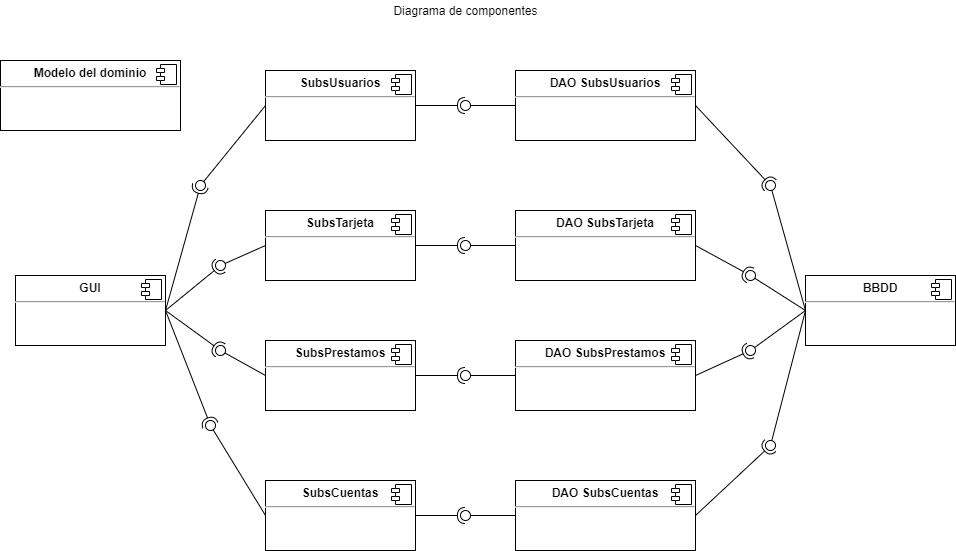
\includegraphics[width=0.8\textwidth]{images/DiagramaDeComponentes.png}
\end{figure}

\newpage
\section{Diagrama de clases para el modelo del dominio}
El diagrama de clases para el modelo del dominio muestra las relaciones existentes entre las clases del programa, además de sus atributos y métodos.
\begin{figure}[H]
    \centering
    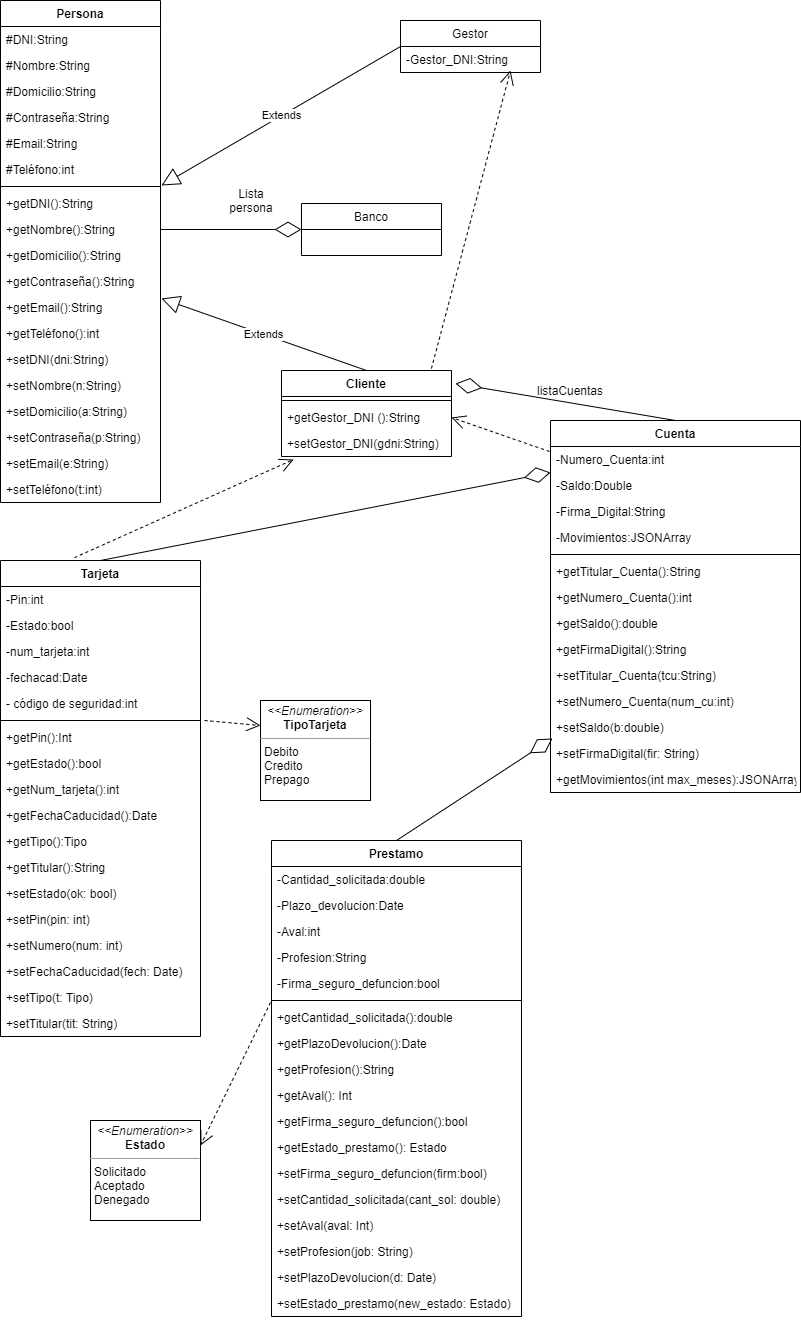
\includegraphics[width=0.8\textwidth]{images/Diagrama_de_clases.png}
\end{figure}

\newpage
\section{Diagrama de clases para la lógica del negocio de cada subsistema}
Los diagramas de clases para la lógica del negocio de cada subsistema recogen los métodos que se hayan en las interfaces de cada uno de ellos, que son los que podrán comunicarse con la Interfaz Gráfica, además de los otros subsistemas.
\subsection{Subsistema de cuentas}
\begin{figure}[H]
    \centering
    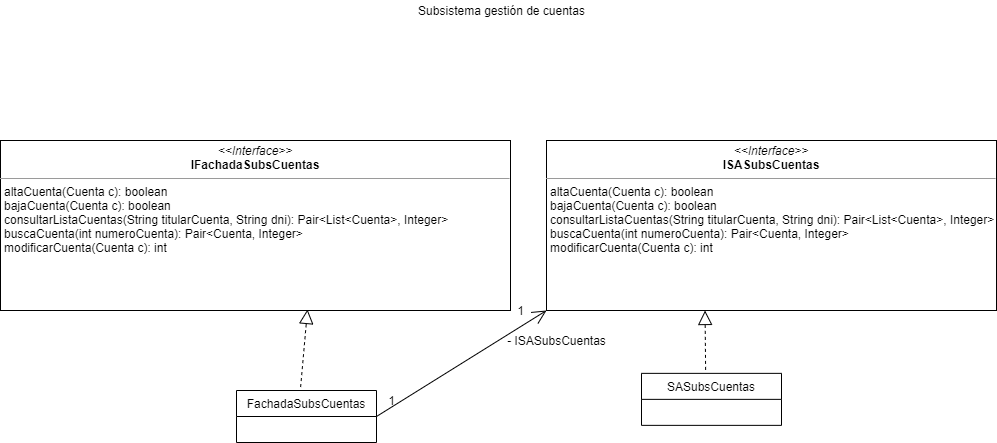
\includegraphics[width=0.8\textwidth]{images/SubsCuentas.png}
\end{figure}
\subsection{Subsistema de préstamos}
\begin{figure}[H]
    \centering
    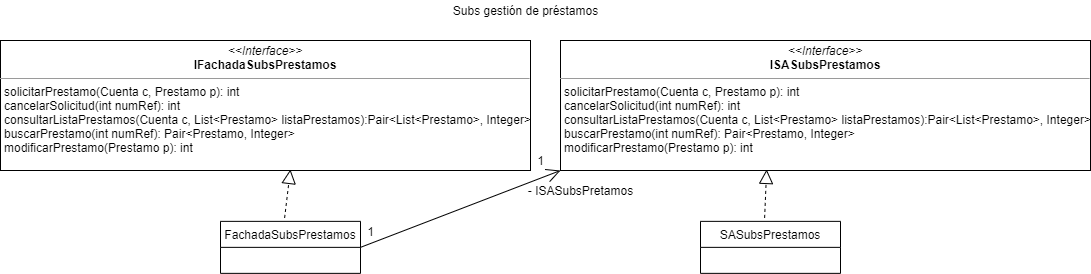
\includegraphics[width=0.8\textwidth]{images/SubsPrestamos.png}
\end{figure}
\subsection{Subsistema de tarjetas}
\begin{figure}[H]
    \centering
    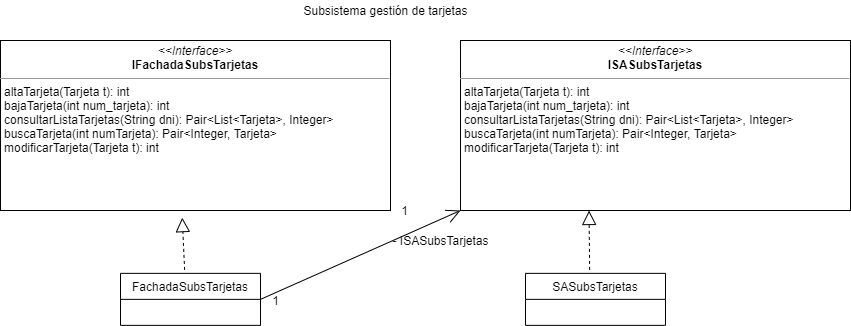
\includegraphics[width=0.8\textwidth]{images/SubsTarjeta.png}
\end{figure}
\subsection{Subsistema de usuarios}
\begin{figure}[H]
    \centering
    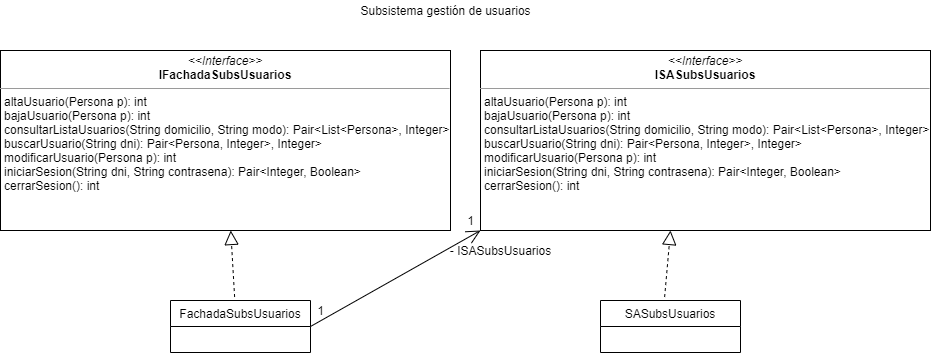
\includegraphics[width=0.8\textwidth]{images/SubsUsuarios.png}
\end{figure}

\newpage
\section{Diagrama de clases para la integración con los datos de cada subsistema}
Los diagramas de clases para la integración con los datos de cada subsistema recogen los métodos que se hayan en las interfaces de los mismos, que son los que podrán comunicarse con la Base de Datos, además de los otros subsistemas.
\subsection{DAO de cuentas}
\begin{figure}[H]
    \centering
    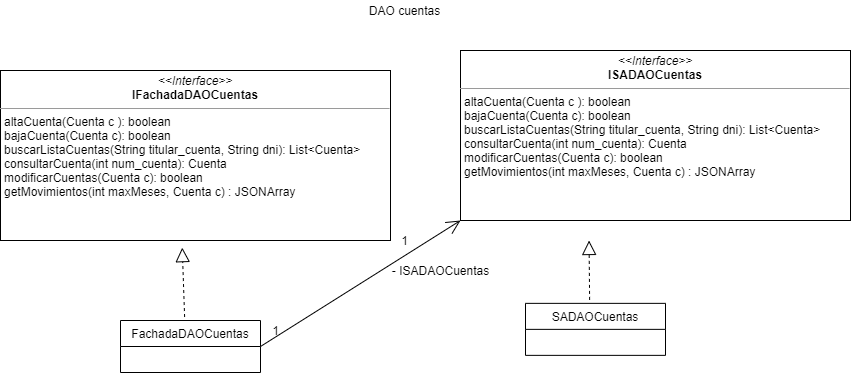
\includegraphics[width=0.8\textwidth]{images/DAOCuentas.png}
\end{figure}
\subsection{DAO de préstamos}
\begin{figure}[H]
    \centering
    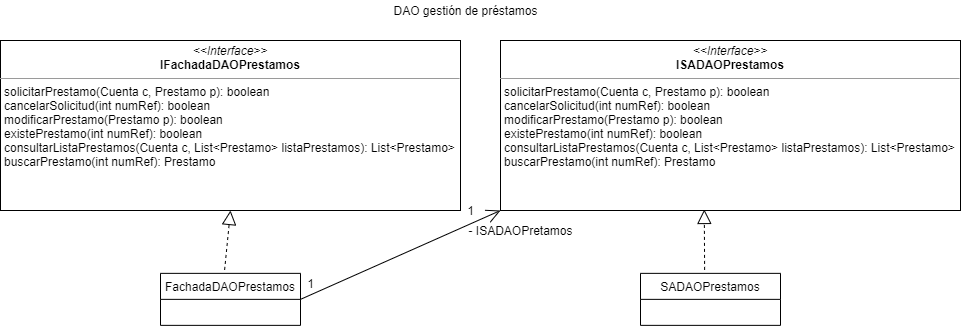
\includegraphics[width=0.8\textwidth]{images/DAOPrestamos.png}
\end{figure}
\subsection{DAO de tarjetas}
\begin{figure}[H]
    \centering
    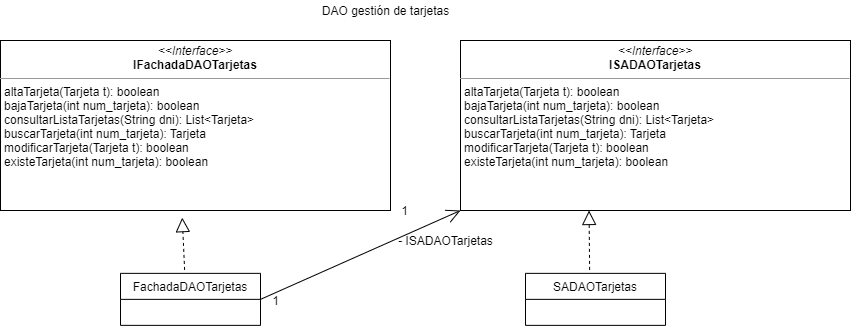
\includegraphics[width=0.8\textwidth]{images/DAOTarjeta.png}
\end{figure}
\subsection{DAO de usuarios}
\begin{figure}[H]
    \centering
    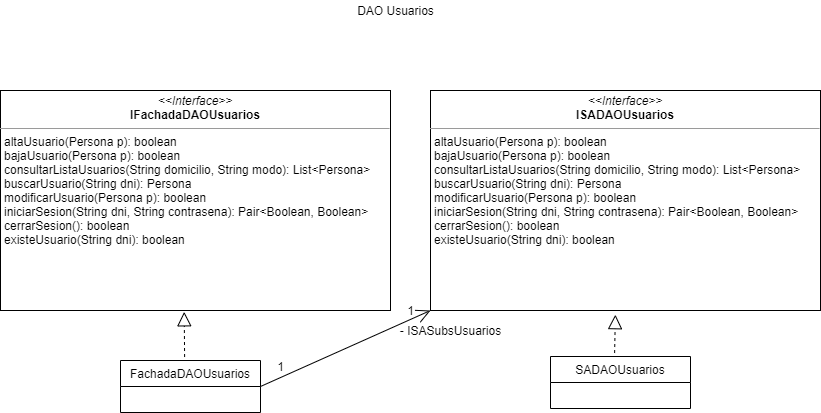
\includegraphics[width=0.8\textwidth]{images/DAOUsuarios.png}
\end{figure}
\end{document}
